\definecolor{c888888}{RGB}{136,136,136}
\definecolor{c808080}{RGB}{128,128,128}

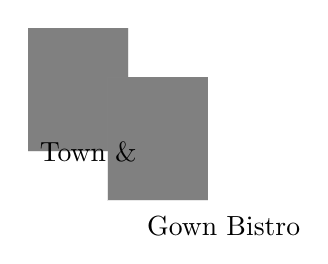
\begin{tikzpicture}[y=0.80pt, x=0.80pt, yscale=-1.000000, xscale=1.000000, inner sep=0pt, outer sep=0pt]
\begin{scope}[shift={(-6.13677,-958.27576)}]
  \path[draw=c888888,fill=c808080,miter limit=4.00,draw opacity=0.196,line
    width=0.400pt,rounded corners=0.0000cm] (6.3868,958.5258) rectangle
    (51.5855,1014.0416);
  \path[draw=c888888,fill=c808080,miter limit=4.00,draw opacity=0.196,line
    width=0.400pt,rounded corners=0.0000cm] (42.2510,980.6338) rectangle
    (87.4497,1036.1496);
  \path[fill=black,line join=miter,line cap=butt,line width=0.800pt]
    (11.6377,1018.9255) node[above right] (text5747) {Town \&};
  \path[fill=black,line join=miter,line cap=butt,line width=0.800pt]
    (60.0746,1052.1510) node[above right] (text5751) {Gown Bistro};
\end{scope}

\end{tikzpicture}
